\begin{frame}{Conservation of Emittance}
\begin{columns}
  \begin{column}{0.42\linewidth}
  \begin{center}
  \begin{tikzpicture}
    \coordinate (spotsize) at (0,2);
    \coordinate (pulselength) at (0.6,0);
    \coordinate (pulse) at (0,0);
    \fill [blue!50, opacity=0.5]
      let
        \p1=(spotsize),
        \p2=(pulselength)
      in
      (pulse)
      ellipse (\x2 and \y1)
    ;
    \node [below=0.3 of pulse] {Pulse (side view)};
    \draw [|-|]
      let 
        \p1 = (spotsize)
      in
      ($(pulse) - (pulselength)$)
      -- node [left, pos=0.5] {$\Delta x$} ++(0,\y1)
    ;
    \draw[-latex, thick]
      (spotsize)
      -- 
        node [pos=0.7] (divangle) {} 
        node [pos=1,above] {$\vec{p}$}
        ++(30:1)
    ;
    \draw[-latex, thick]
      ($(pulse) - (spotsize)$)
      -- node [pos=1,below] {$\vec{p}$} ++(-30:1)
    ;
    \draw[thick, -latex]
      (pulse)
      -- ++(1,0) node [pos=1,label={above left:{$\vec{v_0}$}}] (end v) {}
    ;
    \draw[dashed]
      (end v)
      -- ++(1,0)
    ;
    \draw[latex-latex]
      let
        \p1 = (divangle)
      in
      (divangle)
      arc [
        start angle = 30,
        end angle = 0,
        radius = (\y1 / sin(30))
      ] 
      node [above right] {$\Delta \theta$} 
    ;
  \end{tikzpicture}
  \end{center}
  \end{column}
  \begin{column}{0.56\linewidth}
    \begin{block}<2->{Transverse Normalized Emittance}
      \begin{equation*}
        \varepsilon_{n,x} = \frac{1}{m c} \Delta x \Delta p_{x} 
          = \frac{v_0}{c} \Delta x \Delta \theta
      \end{equation*}
    \end{block}
    \begin{block}<3->{Liouville's Theorem}
      Emittance is conserved under aberration-free propagation
    \end{block}
    \begin{block}<4->{Emittance Growth}	
      Emittance may increase due to aberrations or other adverse conditions
    \end{block}
  \end{column}
\end{columns}
\end{frame}

\begin{frame}{To Improve Resolution}
%For a beam imaged fully on the detector:
  \begin{center}
  \begin{tikzpicture}[scale=0.5]
    \draw (-2,-2) node [below right,align=center] {Detector\\$N_p$ x $N_p$ CCD} rectangle (2,2);
    \draw [step=0.25] (-2,-2) grid (2,2);
    \fill[blue!50, opacity=0.5] (0,0) circle (2);
    \coordinate (lens1) at (-3,0);
    \coordinate (fplane) at (-6,0);
    \coordinate (lens2) at (-7.5,0);

    % beam from sample to detector
    \fill[blue!30, opacity=0.5]
      (0,2) 
      -- ($(lens1) + (0,2)$) 
      -- ($(fplane) + (0,0.1)$)
      -- ($(fplane) - (0,0.1)$)
      -- ($(lens1) - (0,2)$)
      -- (0,-2)
      --cycle;

    % sample
    \draw [fill=yellow!50]
      ($(fplane) + (-0.5,2.1)$)
      -- ++(0,-2)
      -- ++(1,-2)
        node [pos=0.5, pin={[pin distance=1.2cm]below:$\Delta x_s = f_1 \Delta \theta_s$}] {}
      -- ++(0,2)
        node [above=1cm] {Sample} 
      -- cycle
    ;

    % beam from objective to sample
    \fill[blue!30, opacity=0.5]
      ($(lens2) + (0,0.4)$)
      -- ($(fplane) + (0,0.1)$)
      -- ($(fplane) - (0,0.1)$)
      -- ($(lens2) - (0,0.4)$)
      -- cycle
    ;

    % beam spot on sample
    \fill[blue!50, opacity=0.5]
      (fplane) 
      ellipse (0.05 and 0.1)
    ;

    \draw [fill=white] 
      ($(lens1) + (0,3.5)$)
      node [above] {Lenses}
      to [out=262, in=98] ++(0,-7) 
      to [out=82, in=278] ++(0,7)
    ;
    \draw 
      ($(lens1) + (0,3.5)$)
      to [out=273, in=87] ++(0,-7) 
    ;
    \draw [fill=white] 
      ($(lens2) + (0,3.5)$)
      node [above] {Lens ($f_1$)}
      to [out=254, in=106] ++(0,-7)  
      to [out=74, in=286] ++(0,7)
    ;
    \draw 
      ($(lens2) + (0,3.5)$)
      to [out=278, in=82] ++(0,-7) 
    ;
    \fill[blue!30, opacity=0.5]
      ($(lens2) + (-0.4,0.4)$)
      -- ++(-2.5,0)
      node [black,opacity=1,above,pos=0.5] {$\vec{v} \rightarrow$}
      arc [
        start angle=90,
        end angle=270,
        x radius=0.2,
        y radius=0.4
      ]
      -- ++(2.5,0)
      arc [
        start angle=-90,
        end angle=90,
        x radius=0.2,
        y radius=0.4
      ]
    ;
    \fill[blue!50]
      ($(lens2) + (-2.9,0)$) 
      ellipse (0.2 and 0.4)
        node[below=0.4cm,black] {$\Delta x_0 \Delta \theta_0$}
    ;
  \end{tikzpicture}
  %\begin{block}{Resolution}
  %  Resolution = Spot size on sample / 1D Number of Pixels ($N_p$)
  %\end{block}
  %\uncover<2->{Example: 1$\mu$m spot and 1k x 1k CCD $\Rightarrow$ 1nm resolution}
  \end{center}
  \visible<2->{Resolution (per pixel):}
  \begin{equation*}
    \visible<2->{ \Delta X }
    \only<2>{ = \frac{\Delta x_s}{N_p} }
    \only<3->{ = \frac{\sqrt{\Delta x_s^2}}{N_p} }
    \visible<4->{ = \frac{\sqrt{\Delta x_s \Delta \theta_s f_1}}{N_p} }
    \visible<5->{ \ge \frac{\sqrt{\Delta x_0 \Delta \theta_0 f_1}}{N_p} }
  \end{equation*}
\end{frame}

\begin{frame}{Implication of Liouville's Theorem}
  Again results of the previous slides lead to a simple conclusion:
  \vfill
  \begin{block}{}
  \begin{figure}
    \centering
    \begin{tikzpicture} [every node/.style={draw,fill=white,text badly centered,text width=3cm}]
      \node (charges)  {Need a high number of charges};
      \node (child) [below=0.5cm of charges] {Child's law limits charges per area};
      \node (probe) [below=0.5cm of child] {Need a small probe on the sample};
      \node (result1) at ($(charges)!0.5!(child) + (4,0)$) {Need a large emission area};
      \node (emittance) at ($(probe) + (4,0)$) {Need a small transverse emittance};
      \node (result2) at ($(result1)!0.5!(emittance) + (4,0)$) {Need to reduce transverse momentum spread};
      
      \draw [-latex] (charges) -- (result1);
      \draw [-latex] (child) -- (result1);
%      \draw [-latex] (result1.south) to [out=270,in=135] (emittance.north west);
      \draw [-latex] (result1) -- (result2);
      \draw [-latex] (probe) -- (emittance);
      \draw [-latex] (emittance) -- (result2);
    \end{tikzpicture}
  \end{figure}
  \end{block}
  \vfill
\end{frame}

\begin{frame}{Reducing the Transverse Momentum}
  \begin{columns}
    \begin{column}{0.54\linewidth}
    Methods for reducing transverse momentum
    \begin{itemize}
      \item Aperture the beam at a Fourier plane
      \begin{itemize}
        \item<5-> Loss of electrons
        \item<6-> Dynamic lensing at aperture
      \end{itemize}
      \item<7-> Reduce transverse momentum upon emission
    \end{itemize}
    \end{column}
    \begin{column}{0.44\linewidth}
      \begin{center}
      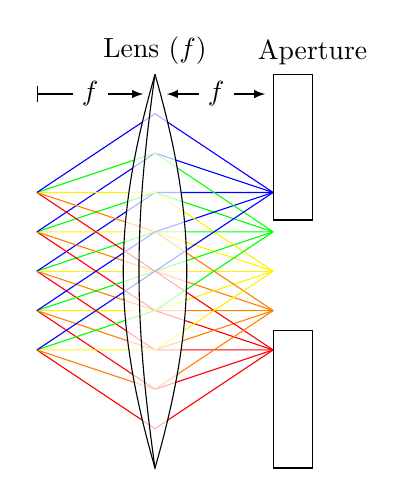
\begin{tikzpicture}[scale=0.5]
        \node (origin) at (0,0) {};
        \foreach \y/\slide in {0/2,1/3,-1/3,2/4,-2/4} {
          \foreach \x/\color in {-2/red, -1/orange, 0/yellow, 1/green, 2/blue} {
            \draw<\slide->[color=\color]
              (0,\y)
              -- ++(3,\x)
              -- (6,\x)
            ;
          }
        }
        \filldraw[fill=white, opacity=0.7, draw=black, draw opacity=1] 
          (3,5)
          node [above,opacity=1] {Lens ($f$)}
          to [out=254, in=106] ++(0,-10)  
          to [out=74, in=286] ++(0,10)
        ;
        \draw 
         (3,5)
          to [out=262, in=98] ++(0,-10) 
        ;
        \draw
          (7,5) node [above] {Aperture}
          rectangle (6,1.3)
        ;
        \draw
          (7,-5)
          rectangle (6,-1.5)
        ;
        \draw [|-latex]
          (0,4.5)
          -- ++(2.7,0)
          node [pos=0.5,fill=white] {$f$}
        ;
        \draw [latex-latex]
          (3.3,4.5)
          -- ++(2.5,0)
          node [pos=0.5,fill=white] {$f$}
        ;
      \end{tikzpicture}
      Transverse momentum reduction by aperturing
      \end{center}
    \end{column}
  \end{columns}
\end{frame}
